\documentclass[12pt,handout,aspectratio=1610]{beamer}
\RequirePackage{
    amsmath,
    amssymb,
    calc,
    cancel,
    booktabs,
    color,
    siunitx,
    tikz,
    wrapfig,
    array,
    leftidx,
    float,
    etoolbox,
    fancyhdr,
    longtable,
    hyperref,
    ltcaption,
    ulem,
    wasysym,
    accents,
    listings,
    tabularx,
}

\hypersetup{
    hidelinks,
    breaklinks              = true,
}

\usepackage[final]{pdfpages}
\usepackage[many]{tcolorbox}

\RenewDocumentCommand{\vec}{m}{\mathbf{#1}}

\makeatletter
    \def\new@mathgroup{\alloc@8\mathgroup\mathchardef\@cclvi}
    \patchcmd{\document@select@group}{\sixt@@n}{\@cclvi}{}{}
    \patchcmd{\select@group}{\sixt@@n}{\@cclvi}{}{}
\makeatother

\RequirePackage{mathspec}                                   % includes fontspec
\RequirePackage{polyglossia}                                % multi-language support
\RequirePackage{xunicode}
\setdefaultlanguage{slovak}

% Setup fonts -- see fontspec/mathspec documentation.
\defaultfontfeatures{
    Mapping         = tex-text,
    Scale           = MatchLowercase,
    Ligatures       = TeX
}


\NewDocumentCommand{\labelmath}{m +m}{%
    \begin{equation}%
        #2%
        \label{#1}%
    \end{equation}%
}

\NewDocumentCommand{\labelalign}{m +m}{%
    \begin{align}%
        #2%
        \label{#1}%
    \end{align}%
}

\linespread{1.0}
\setlength{\parindent}{0cm}
\setlength{\parskip}{6pt}
\setlength{\abovedisplayskip}{0mm}
\setlength{\belowdisplayskip}{0mm}
\setlength{\abovedisplayshortskip}{0mm}
\setlength{\belowdisplayshortskip}{0mm}
\setlength{\itemindent}{0pt}
\setlength{\textfloatsep}{0mm}
\setlength{\tabcolsep}{3mm}
\setlength{\LTcapwidth}{0.8\textwidth}
\renewcommand{\arraystretch}{1.2}

\setcounter{secnumdepth}{2}

/home/kvik/dgs/core/tex/math.tex
\DeclareSIUnit\au{AU}
\DeclareSIUnit\pixel{px}
\DeclareSIUnit\lightyear{ly}
\DeclareSIUnit\parsec{pc}
\DeclareSIUnit\earthmass{M_{\earth}}
\DeclareSIUnit\speedoflight{c}
\DeclareSIUnit\foe{foe}
\DeclareSIUnit\year{yr}
\DeclareSIUnit\eur{€}
\DeclareSIUnit\solarmass{M_{\astrosun}}
\DeclareSIUnit\solarluminosity{L_{\astrosun}}
\DeclareSIUnit{\byte}{B}




\linespread{1.0}
\setlength{\parindent}{0cm}
\setlength{\parskip}{6pt}
\setlength{\abovedisplayskip}{0mm}
\setlength{\belowdisplayskip}{0mm}
\setlength{\abovedisplayshortskip}{0mm}
\setlength{\belowdisplayshortskip}{0mm}
\setlength{\itemindent}{0pt}
\setlength{\textfloatsep}{0mm}
\setlength{\tabcolsep}{3mm}
\renewcommand{\arraystretch}{1.2}

\setcounter{secnumdepth}{0}

\NewDocumentCommand{\fspicture}{m O{W} O{black}}{
    {
        \setbeamertemplate{navigation symbols}{}
        \setbeamercolor{background canvas}{bg = #3}
        \begin{frame}[plain]
            \begin{tikzpicture}[remember picture, overlay]
                \node[at=(current page.center)] {
                    \ifstrequal{H}{#2}{                                  
                        \includegraphics[height=\paperheight]{#1}%
                    }{%
                        \includegraphics[width=\paperwidth]{#1}%
                    }
                };
            \end{tikzpicture}
        \end{frame}
    }
}

\NewDocumentCommand{\frejm}{m +m}{
    \begin{frame}
        \frametitle{#1}
        #2
    \end{frame}
}

\NewDocumentCommand{\fragfrejm}{m +m}{
    \begin{frame}[fragile]
        \frametitle{#1}
        #2
    \end{frame}
}

\defbeamertemplate{description item}{align center}{\hfill\insertdescriptionitem\hfill}
\definecolor{desc}{rgb}{0.66, 0, 0}
\definecolor{citem}{rgb}{0.72, 0, 0}
\definecolor{csitem}{rgb}{0.90, 0, 0}
\definecolor{cssitem}{rgb}{1, 0.1, 0.1}
\definecolor{qprimarybg}{rgb}{0.95, 0.95, 0.95}
\definecolor{check}{rgb}{0, 0.8, 0}
\definecolor{coded}{rgb}{0.9, 0.9, 0.9}
\definecolor{todo}{rgb}{1.0, 0.3, 0.3}
\definecolor{model}{rgb}{0.75, 0, 0}

\setbeamertemplate{navigation symbols}{}
\newfontfamily{\semibold}{Segoe UI Semibold}
\RenewDocumentCommand{\emph}{m}{{\semibold#1}}
\NewDocumentCommand{\code}{m}{\textcolor{desc}{\texttt{#1}}}
\NewDocumentCommand{\model}{m}{\colorbox{coded}{\textcolor{model}{\texttt{#1}}}}
\NewDocumentCommand{\todo}{m}{\colorbox{todo}{#1}}

\mode<presentation> {
    \usetheme{Szeged}
    \usecolortheme{beaver}
    
    \usefonttheme{professionalfonts}
    \setallmainfonts{Minion Pro}
    \setmathrm{Minion Pro}
    
    \setsansfont{Segoe UI}
    \setmonofont{Consolas}
    \setbeamercolor*{enumerate item}{fg = citem}
    \setbeamercolor*{enumerate subitem}{fg = csitem}
    \setbeamercolor*{enumerate subsubitem}{fg = cssitem}
    \setbeamercolor*{description item}{fg = desc}
    \setbeamercolor*{itemize item}{fg = citem}
    \setbeamercolor*{itemize subitem}{fg = csitem}
    \setbeamercolor*{itemize subsubitem}{fg = cssitem}
    \setbeamercolor*{palette primary}{fg = red, bg = qprimarybg}
}

\newcommand<>\highlightbox[2]{%
    \alt#3{\makebox[\dimexpr\width-2\fboxsep]{\colorbox{#1}{#2}}}{#2}%
}

\AtBeginSection[]{
    \subsection{\insertsection}
    \begin{frame}
        \vfill
        \centering
        \begin{beamercolorbox}[sep = 18pt, center, shadow = true, rounded = true]{title}
            \usebeamerfont{title}\insertsectionhead%
            \vfill
        \end{beamercolorbox}
        \vfill
    \end{frame}
}

\makeatletter
% Render percent sign with nice font, not ugly Computer modern
    \mathcode`\%="7025

% Fixes mathspec bug -- URL numbers are rendered with wrong font
    \ernewcommand\eu@MathPunctuation@symfont{Latin:m:n}
    \DeclareMathSymbol{,}{\mathpunct}{\eu@MathPunctuation@symfont}{`,}
    \DeclareMathSymbol{?}{\mathpunct}{\eu@MathPunctuation@symfont}{`?}
    \DeclareMathSymbol{.}{\mathord}{\eu@MathPunctuation@symfont}{`.}
    \DeclareMathSymbol{<}{\mathrel}{\eu@MathPunctuation@symfont}{`<}
    \DeclareMathSymbol{>}{\mathrel}{\eu@MathPunctuation@symfont}{`>}
    \DeclareMathSymbol{/}{\mathord}{\eu@MathPunctuation@symfont}{`/}
    \DeclareMathSymbol{;}{\mathpunct}{\eu@MathPunctuation@symfont}{`;}
    \DeclareMathSymbol{(}{\mathopen}{\eu@DigitsArabic@symfont}{`(}
    \DeclareMathSymbol{)}{\mathclose}{\eu@DigitsArabic@symfont}{`)}
    \XeTeXDeclareMathSymbol{^^^^2026}{\mathinner}{\eu@MathPunctuation@symfont}{"2026}[\mathellipsis]
    \DeclareMathSymbol{0}{\mathalpha}{\eu@DigitsArabic@symfont}{`0}
    \DeclareMathSymbol{1}{\mathalpha}{\eu@DigitsArabic@symfont}{`1}
    \DeclareMathSymbol{2}{\mathalpha}{\eu@DigitsArabic@symfont}{`2}
    \DeclareMathSymbol{3}{\mathalpha}{\eu@DigitsArabic@symfont}{`3}
    \DeclareMathSymbol{4}{\mathalpha}{\eu@DigitsArabic@symfont}{`4}
    \DeclareMathSymbol{5}{\mathalpha}{\eu@DigitsArabic@symfont}{`5}
    \DeclareMathSymbol{6}{\mathalpha}{\eu@DigitsArabic@symfont}{`6}
    \DeclareMathSymbol{7}{\mathalpha}{\eu@DigitsArabic@symfont}{`7}
    \DeclareMathSymbol{8}{\mathalpha}{\eu@DigitsArabic@symfont}{`8}
    \DeclareMathSymbol{9}{\mathalpha}{\eu@DigitsArabic@symfont}{`9}
\makeatother


\sisetup{
    output-decimal-marker = {,},
}

\title{Nobelova cena za fyziku 2019}
\subtitle{James "Jim" Peebles}
\author{Martin Baláž}
\institute{FMFI UK}
\date{2019--10--24}

\begin{document}
    {
        \begin{frame}
            \titlepage
        \end{frame}
    }
                
    \section{Nobelova cena}
        \frejm{James Peebles}{
            {\large ,,For contributions to our understanding of the evolution of the universe and Earth's place in the cosmos``}
            \begin{columns}
                \begin{column}{0.5\textwidth}
                    \begin{itemize}
                        \item 1935, Kanada
                        \item Princeton University
                        \item Einstein Professor of Science
                    \end{itemize}
                \end{column}
                \begin{column}{0.5\textwidth}
                    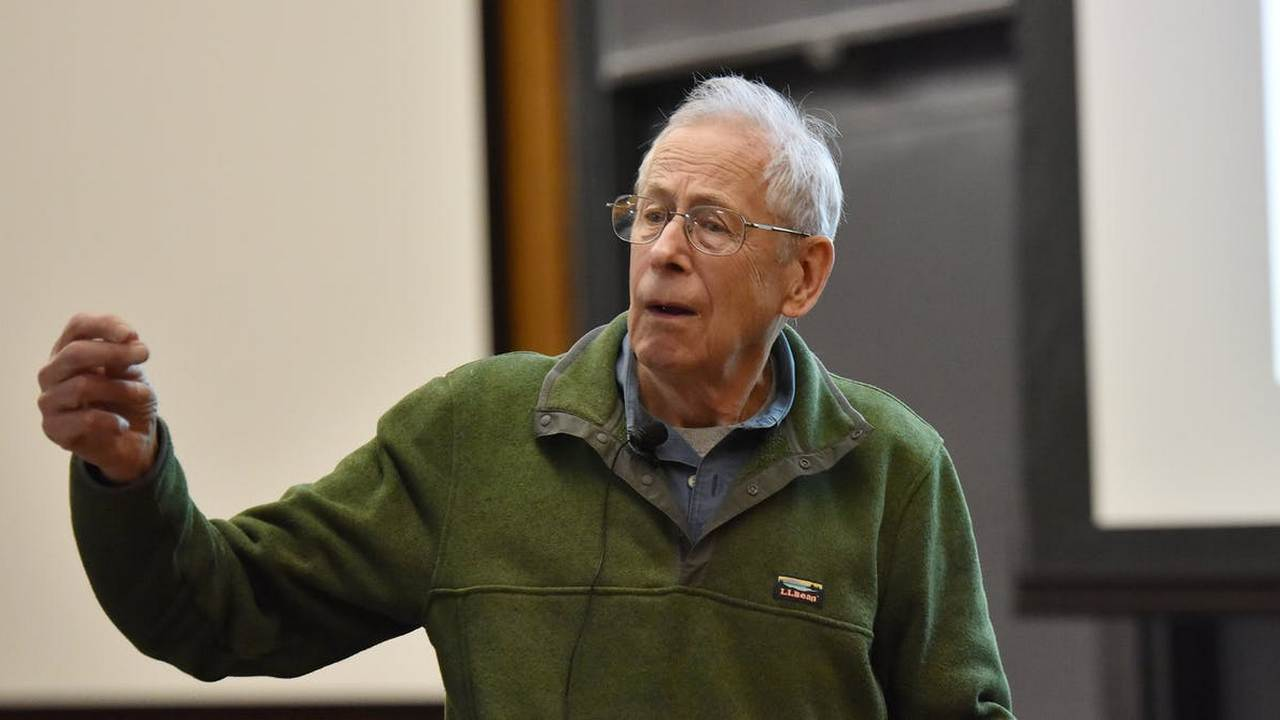
\includegraphics[width = \textwidth]{Peebles.jpg}
                \end{column}
            \end{columns}
        }
        
        \frejm{Dielo}{
            \begin{itemize}
                \item jeden zo zakladateľov modernej kozmológie
                \item Princeton, \emph{Robert Dicke}
                \pause
                \item teoretický pohľad na mladý vesmír
                \pause
                \item celoživotné dielo...
            \end{itemize}
        }


    \section{História}
        \frejm{Expanzia vesmíru}{
            \begin{itemize}
                \item \emph{Edwin Hubble} (1929): červený posun
                \item $\Implies$ čím je galaxia ďalej, tým rýchlejšie sa od nás vzďaľuje
                \pause
                \item vesmír sa rozpína
                \pause
                \item asi \SI{70}{\kilo\metre\per\second\per\mega pc} $\approx$ \num{2.2e-18}
            \end{itemize}
        }

        \frejm{Veľký tresk}{
            \begin{itemize}
                \item \emph{George Gamow} a \emph{Georges Lemaître}
                \pause
                \item poďme späť v čase
                \item ak sa vesmír rozpína, kedysi musel byť menší a horúcejší
                \pause
                \item asi pred \SI{1.38e-10}{rokov} musel byť takmer bodový
            \end{itemize}
        }
        
        \fspicture{inflation.jpg}

        \frejm{Expanzia vesmíru}{
            \begin{columns}
                \begin{column}{0.5 \textwidth}
                    \begin{itemize}
                        \item asi 380000 rokov po Veľkom tresku
                        \item teplota klesá pod \SI{3000}{\kelvin}
                        \pause
                        \item formujú sa neutrálne atómy
                        \item vesmír je priehľadný
                    \end{itemize}
                    \pause
                    \begin{itemize}
                        \item svetlo sa môže voľne šíriť
                        \item expanzia, červený posun...
                        \pause
                        \item dnes asi 1100-krát menej, \SI{2.725}{\kelvin}
                        \item žiarenie čierneho telesa
                    \end{itemize}
                \end{column}
                \begin{column}{0.5 \textwidth}
                    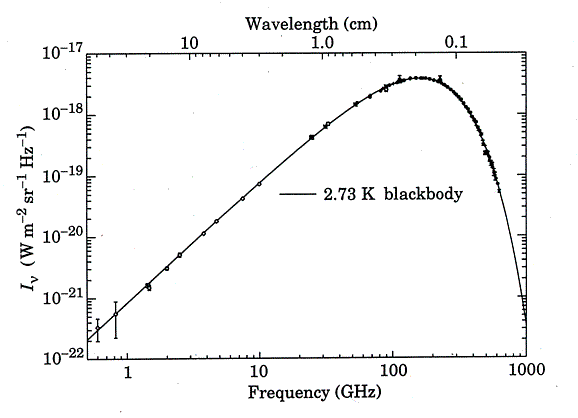
\includegraphics[width = \textwidth]{spectrum.png}
                \end{column}
            \end{columns}
        }

        \frejm{Objav}{
            \begin{itemize}
                \item \emph{Arno Penzias} a \emph{Robert Wilson}, 1964
                \item Holmdel Horn Antenna
                \pause
                \item holuby v anténe...
                \pause
                \item prvé priame pozorovanie CMB (Dicke)
                \item Nobelova cena za fyziku 1978
            \end{itemize}
        }
        
        \fspicture{Holmdel.jpeg}
        \fspicture{WMAP_2010.png}

        \frejm{Tmavá hmota + energia}{
            \begin{columns}
                \begin{column}{0.5 \textwidth}
                    \begin{itemize}
                        \item expanzia vesmíru sa \emph{zrýchľuje}
                        \pause
                        \item \emph{ΛCDM model}
                        \item vesmír je homogénny a izotropný
                        \item odchýlky sú viditeľné vo WMAP
                    \end{itemize}
                \end{column}
                \begin{column}{0.5 \textwidth}
                    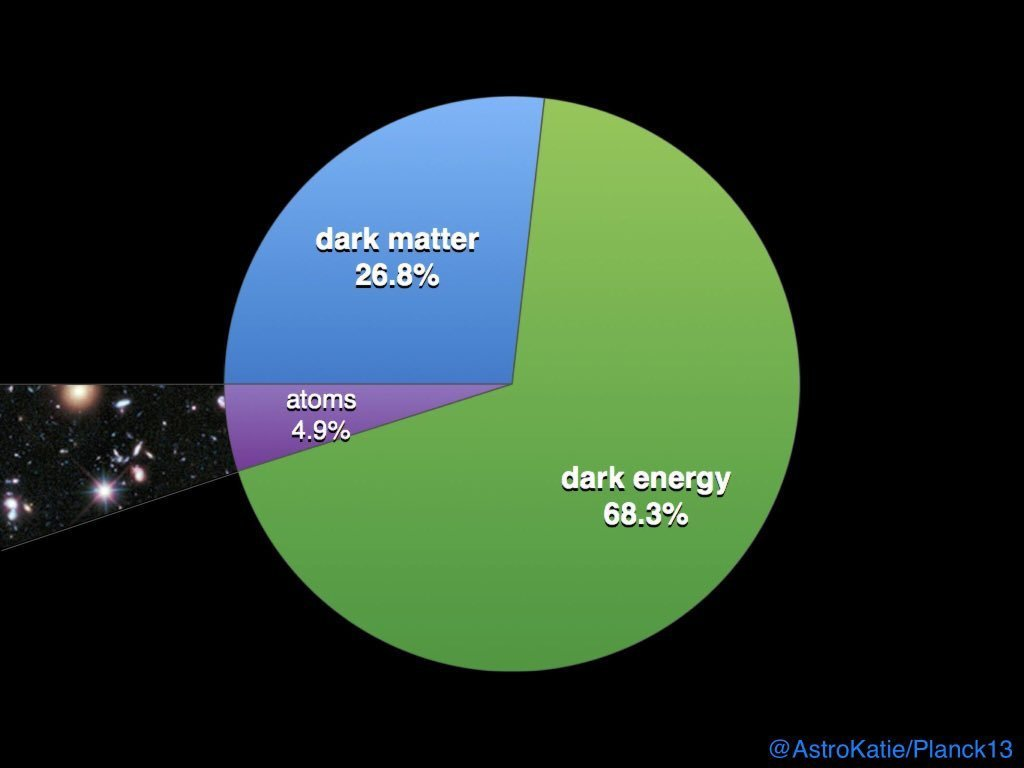
\includegraphics[width = \textwidth]{pie.jpg}
                \end{column}
            \end{columns}
        }

        \fspicture{cosmic-web.jpg}

    \section{Alternatívne teórie}
        \frejm{Bez tmavej hmoty}{
            Veľa pozorovaní sa dá vysvetliť aj inak...
            \begin{itemize}
                \item rotačné krivky galaxií (\emph{Zwicky} 1930)
                \item gravitačné šošovkovanie
            \end{itemize}
        }

        \fspicture{rotation-curve.png}

        \frejm{MOND}{
            \begin{itemize}
                \item Čo ak je gravitácia iná?
                \item \emph{Milgrom} 1983
            \end{itemize}
            $$
                \cancel{\vec{F} = Gm_1m_2 \frac{\vec{r}}{r^3}}
            $$
            \pause
            $$
                \vec{F} = \frac{G m_1 m_2}{1 - \exp\left(-\sqrt{\frac{g}{g+}}\right)} \frac{\vec{r}}{r^3}
            $$
            \begin{itemize}
                \item $g+ \approx \SI{1.2e-10}{\metre\per\second\squared}$
            \end{itemize}
        }
        
        \frejm{Referencie}{
            \begin{itemize}
                \item NASA (WMP 2010, Holmdel Horn Antenna)
                \item Princeton University/EPA (James Peebles)
                \item Mario de Leo (Rotation curves)
            \end{itemize}
        }
            
\end{document}
